
\begin{minipage}{0.5\linewidth}
Le graphique ci-dessous montre les résultats à un contrôle de sciences obtenus par deux groupes d'élèves, désignés par « Groupe A » et « Groupe B ». 
La note moyenne pour le Groupe A est de 62,0 et de 64,5 pour le Groupe B. Les élèves réussissent ce contrôle lorsque leur note est de 50 points ou davantage. Sur la base de ce graphique, le professeur conclut que le Groupe B a mieux réussi ce contrôle que le Groupe A. Les élèves du Groupe A ne sont pas d'accord avec le professeur. Ils essaient de le convaincre que le Groupe B n'a pas nécessairement mieux réussi. \hfill{{\scriptsize D'après PISA 2009}}
\end{minipage}
\begin{minipage}{0.5\linewidth}
\begin{center}
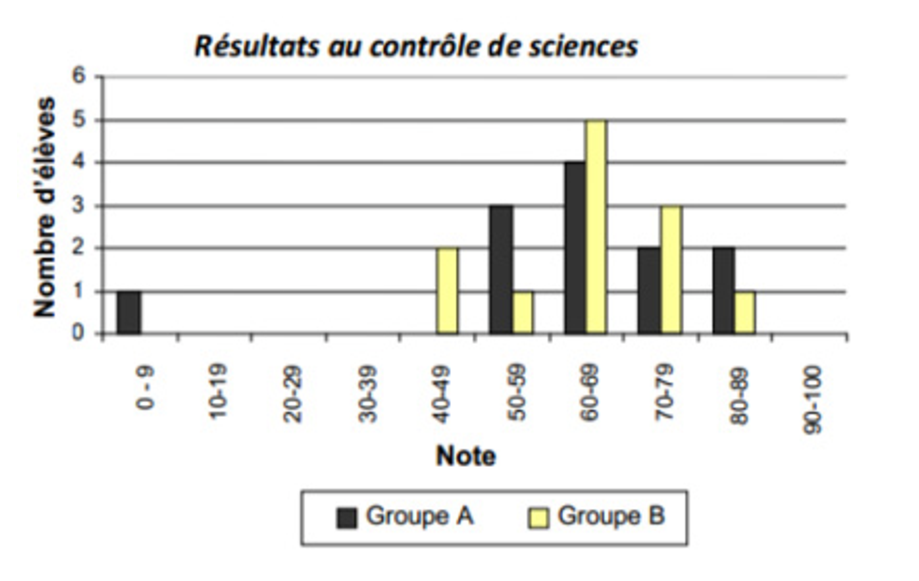
\includegraphics[scale=0.6]{Stat-13.eps} 
\end{center}
\end{minipage}
En vous servant du graphique, donnez un argument mathématique que les élèves du Groupe A pourraient utiliser. 

